% Assembled-window-regions figure for Ch9 ("The assembled window").
% Standalone TikZ; compiled by `book-scaffold build-figures` via pdflatex -> pdftocairo -> SVG.
% Three positional regions (stable front -> volatile tail) under a U-shaped attention curve.
\documentclass[tikz,border=4mm]{standalone}
\usepackage{tikz}
\usetikzlibrary{positioning, arrows.meta, calc}

\begin{document}
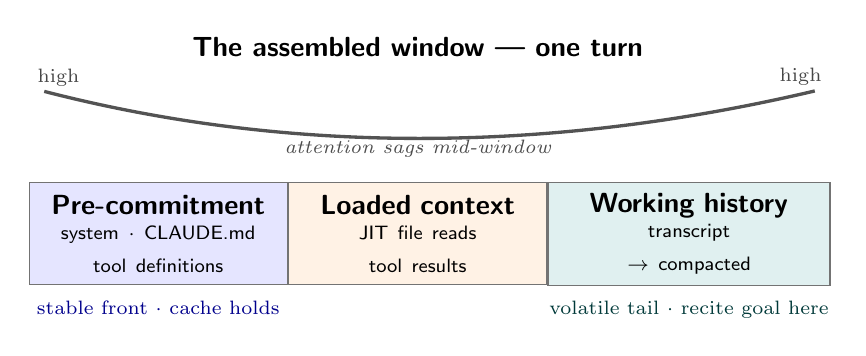
\begin{tikzpicture}[
  font=\sffamily,
  region/.style={draw=black!55, align=center, minimum height=1.3cm, inner sep=4pt},
  lbl/.style={font=\scriptsize},
]

% --- the window bar: three regions, front (left, stable) -> tail (right, volatile)
\node[region, fill=blue!10,   text width=3.0cm] (p)
  {\textbf{Pre-commitment}\\[1pt]{\scriptsize system $\cdot$ CLAUDE.md\\ tool definitions}};
\node[region, fill=orange!10, text width=3.0cm, right=0pt of p] (l)
  {\textbf{Loaded context}\\[1pt]{\scriptsize JIT file reads\\ tool results}};
\node[region, fill=teal!12,   text width=3.3cm, right=0pt of l] (h)
  {\textbf{Working history}\\[1pt]{\scriptsize transcript\\ $\to$ compacted}};

% --- front / tail annotations under the bar
\node[lbl, text=blue!55!black, below=2pt of p.south] {stable front $\cdot$ cache holds};
\node[lbl, text=teal!45!black, below=2pt of h.south] {volatile tail $\cdot$ recite goal here};

% --- U-shaped attention curve above the bar (high at the edges, sags mid-window)
\coordinate (cl) at ($(p.north west)+(0.2,1.15)$);
\coordinate (cr) at ($(h.north east)+(-0.2,1.15)$);
\draw[very thick, draw=gray!65!black]
  (cl) .. controls ($(p.north east)+(0,0.35)$) and ($(h.north west)+(0,0.35)$) .. (cr);
\node[lbl, text=gray!55!black] at ($(cl)+(0.18,0.18)$) {high};
\node[lbl, text=gray!55!black] at ($(cr)+(-0.18,0.18)$) {high};
\node[lbl, font=\scriptsize\itshape, text=gray!60!black] at ($(l.north)+(0,0.42)$) {attention sags mid-window};

% --- title
\node[font=\sffamily\bfseries] at ($(l.north)+(0,1.72)$) {The assembled window --- one turn};

\end{tikzpicture}
\end{document}
